\documentclass[12pt,twoside,a4paper]{article}
\usepackage{amsmath, amssymb, amsfonts, mathrsfs} %les plus utiles et quasi indispensables 
\usepackage{amsthm}%\usepackage[T1]{fontenc}
\usepackage{a4wide}
\usepackage[utf8]{inputenc}
\usepackage{fancyhdr} %pour les hauts et bas de page
\usepackage[francais]{babel}% donne de bonnes c\'esures  en francais
\usepackage{titlesec}%pour modifier le style des sections
\usepackage{float}%pour fixer les flottants
\usepackage{url}%pour ecrire une adresse d'un site web
\usepackage[all]{xy}%pour faire des diagrammes
\usepackage[dvips]{graphicx}
\usepackage{todonotes}
\usepackage{graphicx}
\usepackage{pgf,tikz}
\usetikzlibrary{arrows}
\usepackage{enumitem}
\usepackage[T1]{fontenc}
\usepackage{hyperref}
\usepackage{array}
\usepackage{chemfig}
\usepackage{graphics}
\usepackage{eurosym}
\usepackage{soul}
\usepackage{wasysym}
\usepackage{textcomp}
\usepackage{listings}
\usepackage{stmaryrd}



\title{TDLog : Jelly-game}
\author{\textsc{BATY L\'eo, BRUNOD-INDRIGO Luca, CAMPO Yannis,}\\ \textsc{LAURET J\'eremy, LO Emmanuel}}
\date{15/02/2019}


\begin{document}
\maketitle

\tableofcontents

\newpage%%%

\section{Objectifs initiaux}
\todo[inline]{blabla \`a \'ecrire}

\newpage%%%

\section{Organisation/architecture du code}
\todo[inline]{(i.e. ce qui n'est pas dans le code, mais nécessaire à sa compréhension)}

Nous avons utilis\'e un backend en python avec le framework Django, et un frontend ReactJs.

\subsection{Backend Django}

\begin{figure}[H]
\centering
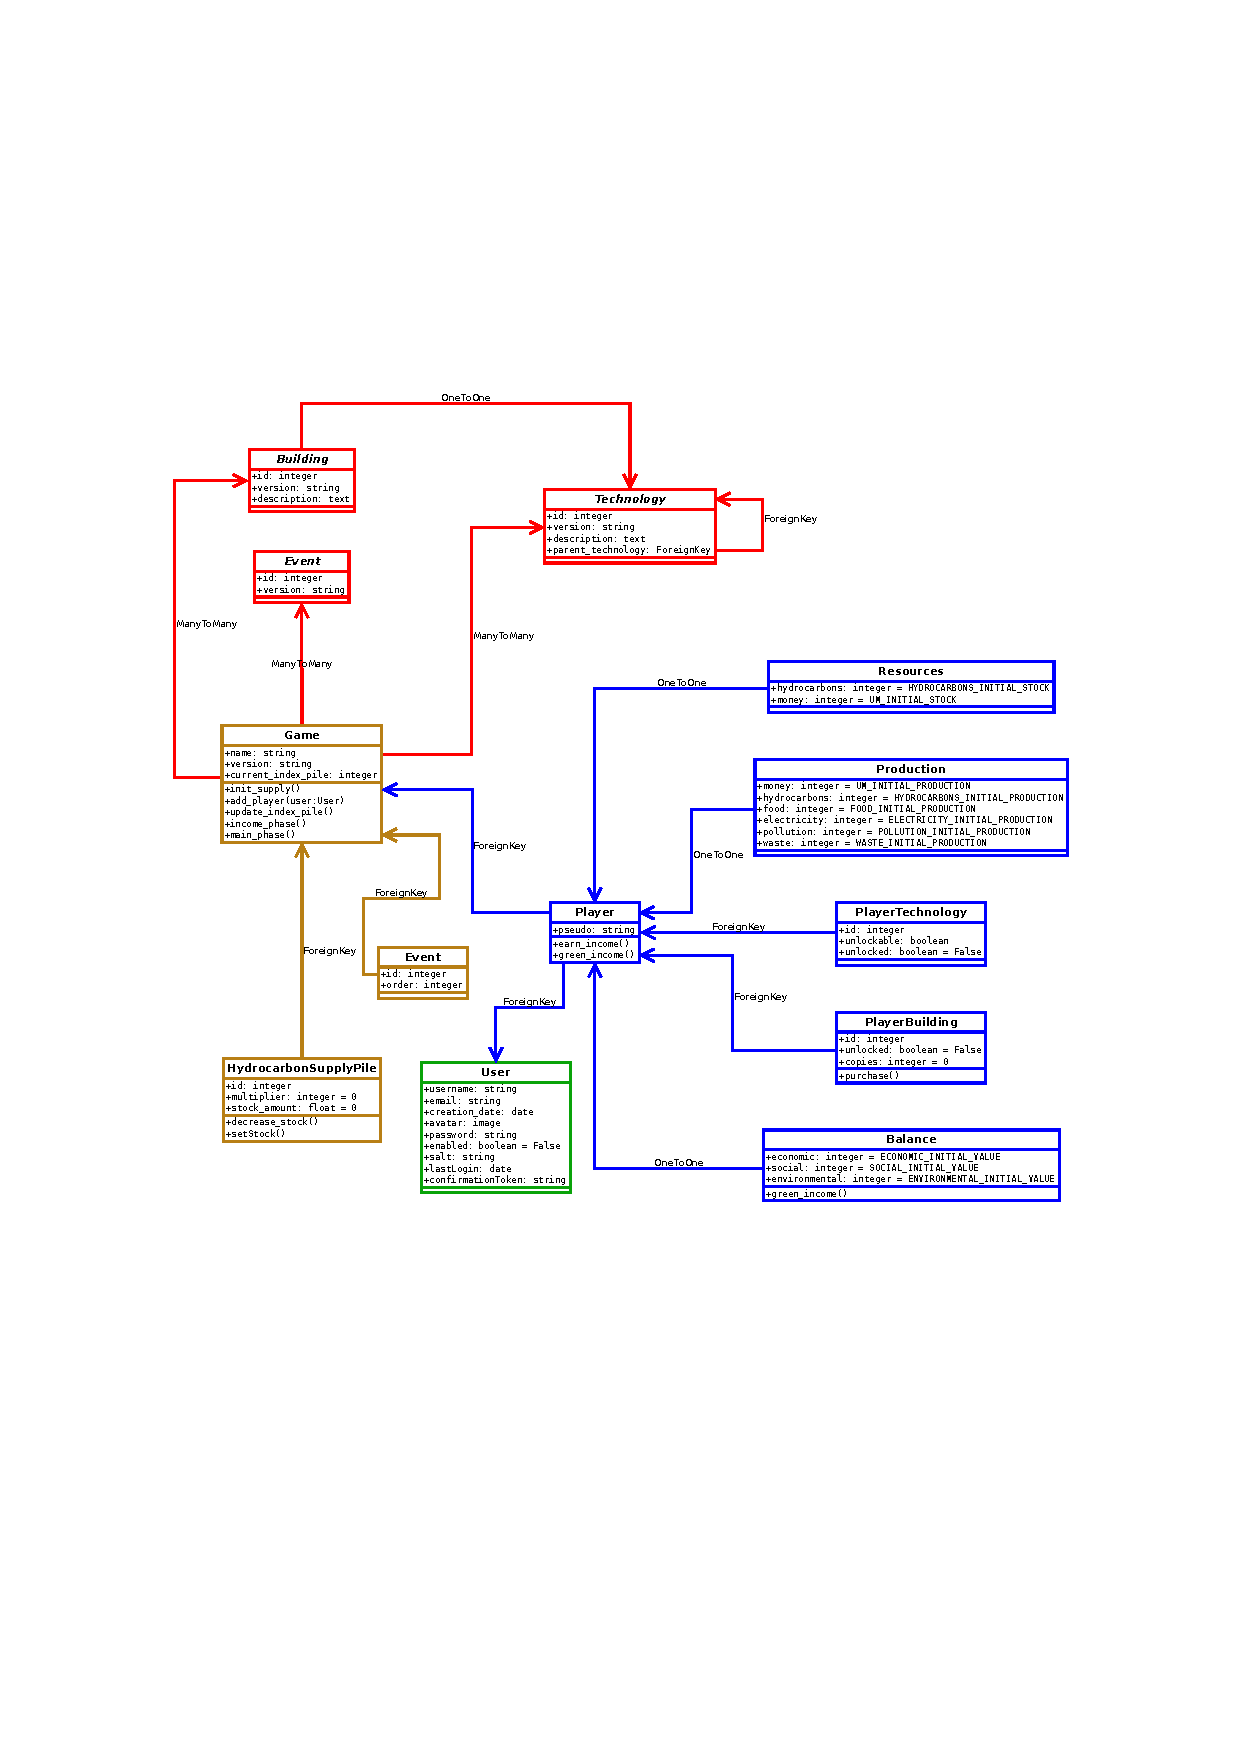
\includegraphics[width=15cm]{../global_uml.pdf}
\caption{Diagramme UML des mod\`eles}
\end{figure}

\subsection{Frontend React}

\section{El\'ements r\'ealis\'es}
\todo[inline]{(il est usuel d'avoir un delta avec les objectifs initiaux)}

\section{Probl\`emes r\'ealis\'es}
\todo[inline]{(afin que nous capitalisions de l'expérience en vue des prochaines promos)}






\end{document}